\documentclass[letterpaper, 11pt]{article}
\usepackage{nopageno} % For removing page numbers
\usepackage[utf8]{inputenc}
\usepackage{color, colortbl} % For table coloring
\usepackage{titling} % For positioning of title preamble
\usepackage[margin=0.75in]{geometry} % For margin width setting
\usepackage{comment} % For block commenting
\usepackage{float} % For table positioning
% For math equation formatting
\usepackage{amsmath, amssymb, amsfonts}
\newcommand{\PMod}[1]{\ (\mathrm{mod}\ #1)}
\newcommand{\Mod}[1]{\ \mathrm{mod}\ #1}
\usepackage{parskip} % For automatic paragraph spacing/formatting
\usepackage{relsize} % For increased math mode font sizing
% For code blocks
\usepackage[dvipsnames,table]{xcolor}
\usepackage[most]{tcolorbox}
\usepackage{lmodern}
\renewcommand{\ttdefault}{lmtt}
\usepackage{listings, minted}
\lstset{
    basicstyle=\ttfamily\footnotesize,
    keepspaces=false,
    showstringspaces=false,
    keywordstyle=\color{blue},
    commentstyle=\sffamily\itshape\color{Green}\scriptsize,
    stringstyle = \color{red},
    breaklines=true,
    breakatwhitespace=false,
    tabsize=2
}
\tcbset{
    colback=gray!5!white,
    colframe=gray!75!black,
    oversize,
    parbox=false,
}
\setlength{\extrarowheight}{2pt}
\usepackage{titlesec} % Custom styling for section titles
\titleformat{\section}
  {\normalfont\LARGE\bfseries}{\thesection}{1em}{}
\titleformat{\subsection}
  {\normalfont}{\thesection}{1em}{}
% For side by side figures
\usepackage{multicol}
\usepackage{makecell}
% For horizontal lists
\usepackage{enumitem, tasks, varwidth}
% For custom page numbers
\usepackage{fancyhdr, lastpage}
\pagestyle{fancy}
\fancyhead{}
\fancyfoot{}
\renewcommand{\headrulewidth}{0pt}
\usepackage[skip=2pt]{caption}
\usepackage{graphicx}
\graphicspath{{../Images/}}

% Move title area to the top of the page
\setlength{\droptitle}{-4em}
\addtolength{\droptitle}{-4pt} 
\renewcommand{\arraystretch}{1.25}
% Disable paragraph indenting
\setlength{\parindent}{0pt}

\usepackage[none]{hyphenat}
\usepackage{times}
\usepackage{soul}

\title{Midterm Prep: Relational Algebra and SQL}
\author{}
\date{}

\begin{document}

\maketitle

\vspace{-4em}

\section*{Question 1}

Consider a database which keeps track of customers and the hotels that they stay at. A customer has an identifier (\texttt{cid}). A customer also has a name, city, state, date of birth, and phone number. Customers stay at hotels. Hotels also have a unique identifier. In addition, they have name, city, and state. Hotels also are rated with a star rating.

\begin{enumerate}[label={\alph*}.,leftmargin=*]
    \item Draw the EF diagram for the above description.
    \begin{tcolorbox}
    \begin{figure}[H]
        \centering
        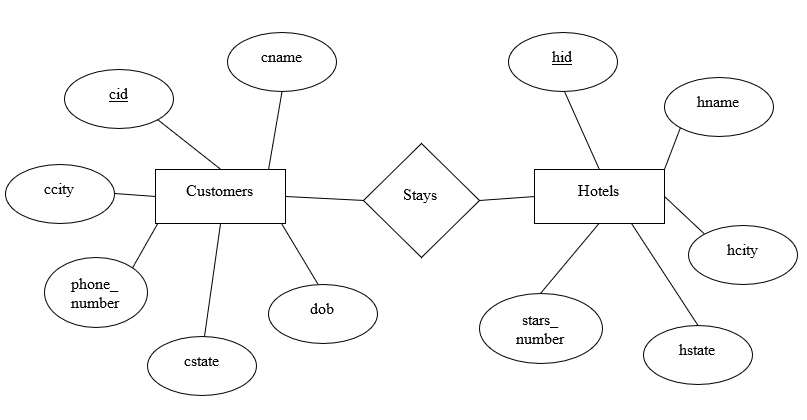
\includegraphics[scale=0.8]{midterm-1a.png}
    \end{figure}
    \end{tcolorbox}
    \item Write the DB schema for the above description.
    \begin{tcolorbox}
    \begin{itemize}[leftmargin=*]
        \item \textit{Customers} (\ul{\texttt{cid}: int}, \texttt{cname}: string, \texttt{ccity}: string, \texttt{cstate}: string, \texttt{dob}: date, \texttt{phone\_number}: string)
        \item \textit{Hotels} (\ul{\texttt{hid}: int}, \texttt{hname}: string, \texttt{hcity}: string, \texttt{hstate}: string, \texttt{star\_rating}: int)
        \item \textit{Stays} (\ul{\texttt{cid}: int, \texttt{hid}: int})
    \end{itemize}
    \end{tcolorbox}
\end{enumerate}

\section*{Question 2}

Given the following DB schema:
\begin{itemize}
    \item \textit{Musicians} (\ul{\texttt{mid}: int}, \texttt{name}: string, \texttt{city}: string, \texttt{state}: string, \texttt{dob}: date, \texttt{rating}: real)
    \item \textit{Instruments} (\ul{\texttt{iid}: int}, \texttt{brand}: string, \texttt{model}: string, \texttt{myear}: int, \texttt{category}: string, \texttt{dailyfee}: real)
    \item \textit{Rents} (\ul{\texttt{mid}: int, \texttt{iid}: int})
\end{itemize}

\begin{enumerate}[label={\alph*}.,leftmargin=*]
    \item Get the id, name, and city of all musicians that are from MA.
    
    \begin{tcolorbox}
    \[\pi_{\textit{mid,name,city}}\left(\sigma_{\textit{state}=\textit{`MA'}}\textit{Musicians}\right)\]
    \end{tcolorbox}
    
    \item Get the id and name of the musicians and the id and category of the instruments they rented.

    \begin{tcolorbox}
    \[\pi_{\textit{mid,name,iid,category}}\left(\textit{Musicians} \bowtie \textit{Rents} \bowtie \textit{Instruments}\right)\]
    \end{tcolorbox}

    \item Get the id and name of musicians that rented instruments of the category guitar and piano.
    \begin{tcolorbox}
    \[\rho\left(\textit{GuitarRentals}, \pi_{\textit{mid,name}}\left(\textit{Musicians} \bowtie \textit{Rents} \bowtie \left(\sigma_{\textit{category}=\textit{`guitar'}}\textit{Instruments}\right)\right)\right)\]
    \[\rho\left(\textit{PianoRentals}, \pi_{\textit{mid,name}}\left(\textit{Musicians} \bowtie \textit{Rents} \bowtie \left(\sigma_{\textit{category}=\textit{`piano'}}\textit{Instruments}\right)\right)\right)\]
    \[\textit{GuitarRentals} \cap \textit{PianoRentals}\]
    \end{tcolorbox}
\end{enumerate}

\section*{Question 3}

Write the SQL statements for the following queries given the schema used for Question 2.

\begin{enumerate}[label={\alph*}.,leftmargin=*]
    \item The information of musicians whose name contains the string `an'.
    \item The number of musicians for all ratings in the database.
    \item Save the id, name, city, and state of the youngest musicians into a view called \textit{YoungestMusicians}.
    \item The id, brand, and model of all instruments that were manufactured in the year 2020 from either `yamaha' or `roland' (which are brands).
    \item The average daily fee for each instrument category in the database. Only keep categories that have more than 3 instruments.
    \item The id and name of musicians that only rented pianos.
    \item The total amount of daily fees for all instruments that have been rented by each musician in the database. Also, include the id and name of the musicians.
    \item Add a phone number column to the \textit{Musicians} table.
    \item Explain the primary key constraint. How is it used in databases? How does it affect the creation and altering of data? Show an example of a violation of this constraint.
\end{enumerate}

\end{document}
